% =====================================================================
\chapter{Resultados}\label{cap:resultados}
% =====================================================================

Todas las simulaciones usan el código del repositorio del proyecto \parencite{repo2026},
escrito en PyTorch \parencite{paszke2019} con el propagador de banda limitada del
\cref{cap:numerico}. Los dígitos provienen de la base MNIST \parencite{lecun1998}. Las
decisiones que el artículo no especifica se resumen en \cref{tab:decisiones}
(\cref{ap:implementacion}).

\section{Reproducción de la Fig.~6 del artículo}\label{sec:fig6}

Se entrenó la red reducida ($80\times80$ neuronas, 5 capas, 10 clases) en las configuraciones
de \cref{tab:casos}, con \num{10000} imágenes de entrenamiento, 500 de prueba, Adam con tasa
de aprendizaje \num{e-3} y 20 épocas. Cada caso tarda unos \SI{2.5}{min} en un procesador de
cuatro núcleos. \Cref{tab:fig6} compara las precisiones con las del artículo y \cref{fig:fig6b}
sitúa los casos respecto a la curva \eqref{eq:dmin}.

\begin{table}[htbp]
\centering
\caption[Reproducción de la Fig.~6(c) del artículo]{Precisión de prueba de la red
reducida ($80\times80$) en los casos de la Fig.~6(c) de \textcite{chen2021}.}
\label{tab:fig6}
\begin{tabular}{@{}lccccc@{}}
\toprule
Caso & $d_f$ ($\lambda$) & $D$ ($\lambda$) & $D/\Dmin$ & Artículo (\%) & Este trabajo (\%)\\
\midrule
1 & 0.53 & 15 & 1.01 & 90.0 & \textbf{89.8}\\
2 & 6 & $5.7\times10^3$ & 0.99 & 91.0 & \textbf{89.0}\\
3 (valor de la gráfica) & 6 & $2.4\times10^4$ & 4.18 & 91.2 & 84.8\\
3 (valor de la tabla) & 6 & $2.4\times10^3$ & 0.42 & 91.2 & \textbf{91.2}\\
4 & 12 & 15 & \num{6.5e-4} & ``$\sim$0.1'' & 14.4\\
\bottomrule
\end{tabular}
\end{table}

\begin{figure}[htbp]
\centering
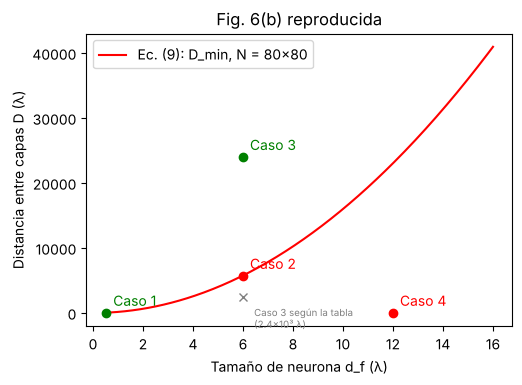
\includegraphics[width=0.62\textwidth]{e_fig6b_curva.png}
\caption[Curva de conectividad y casos de prueba]{Reproducción de la Fig.~6(b) de
\textcite{chen2021}: curva $\Dmin(d_f)$ de \cref{eq:dmin} para $\sqrt N=80$ y los cuatro
casos. Se marcan los dos valores del caso~3 que aparecen en el artículo.}
\label{fig:fig6b}
\end{figure}

\begin{figure}[htbp]
\centering
\begin{subfigure}{0.45\textwidth}\centering
  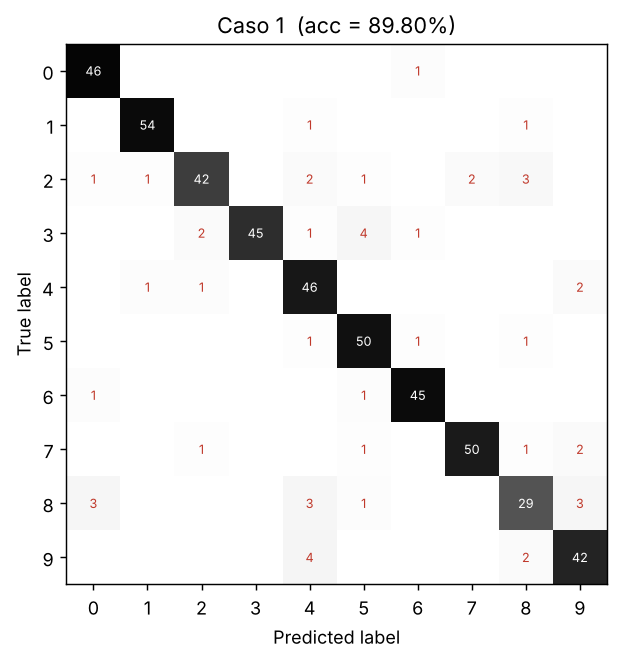
\includegraphics[width=\textwidth]{confusion_caso1.png}\caption{Caso 1}\end{subfigure}\hfill
\begin{subfigure}{0.45\textwidth}\centering
  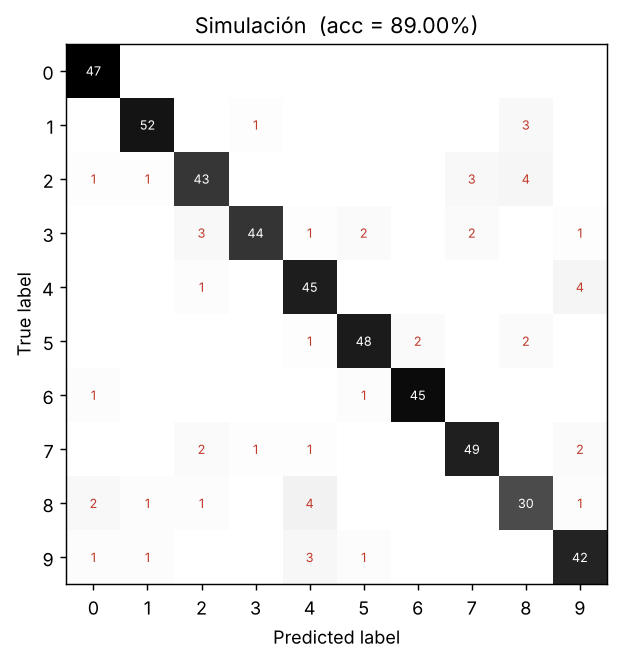
\includegraphics[width=\textwidth]{confusion_caso2.png}\caption{Caso 2}\end{subfigure}\\[4pt]
\begin{subfigure}{0.45\textwidth}\centering
  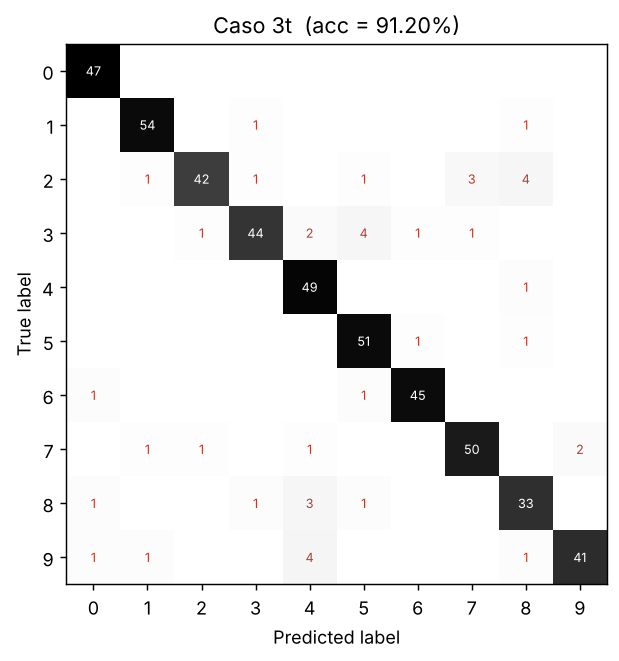
\includegraphics[width=\textwidth]{confusion_caso3_tabla.png}\caption{Caso 3 (valor de la tabla)}\end{subfigure}\hfill
\begin{subfigure}{0.45\textwidth}\centering
  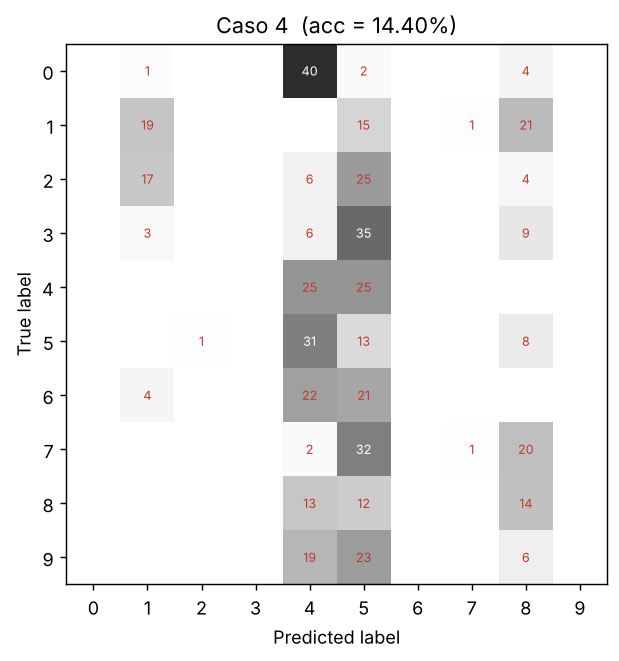
\includegraphics[width=\textwidth]{confusion_caso4.png}\caption{Caso 4}\end{subfigure}
\caption[Matrices de confusión de los casos de la Fig.~6]{Matrices de confusión sobre las
500 imágenes de prueba, equivalentes a las Figs.~6(d)--(g) del artículo. En el caso~4 las
predicciones se concentran en pocas columnas, como en la Fig.~6(g) original.}
\label{fig:confusiones}
\end{figure}

Los casos~1 y~2 se reproducen con una diferencia de 0.2 y 2 puntos porcentuales. El caso~4,
con neuronas grandes y capas muy próximas, no aprende: con $\varphi_{\max}=\ang{2.39}$ y
$D=15\lambda$, la luz se desplaza lateralmente $R=D\tan\varphi_{\max}\approx0.6\lambda$, menos de una
neurona. Cada capa sólo cambia la fase local, y una máscara de solo fase no modifica la
intensidad local; la distribución de intensidad en la salida es prácticamente la de la
entrada, sin importar cómo se entrenen las fases.

\FloatBarrier
\section{Inconsistencias en el artículo}\label{sec:inconsistencias}

\begin{enumerate}
  \item \textbf{El caso~3.} Con la distancia de la gráfica ($2.4\times10^4\lambda$, encima de la
  curva) se obtiene \SI{84.8}{\percent}; con la de la tabla ($2.4\times10^3\lambda$, debajo de la
  curva) se obtiene \SI{91.2}{\percent}, que coincide exactamente con el valor que reporta el
  artículo. Lo más probable es que la tabla sea la correcta y el punto de la gráfica esté mal
  colocado. En ese caso, el propio artículo contiene una configuración ``no totalmente
  conectada'' ($D=0.42\,\Dmin$) que funciona tan bien como las conectadas, lo que
  contradice la lectura de \eqref{eq:dmin} como condición necesaria.
  \item \textbf{El caso~4.} Una precisión de ``$\sim$\SI{0.1}{\percent}'' es imposible: el azar con
  10 clases da \SI{10}{\percent}. La matriz de confusión del artículo corresponde a una precisión
  de ese orden, así que el valor debe leerse como la fracción $0.1$. Aquí se obtiene
  \SI{14.4}{\percent}.
  \item \textbf{Alejar las capas no es gratis.} Con $D=4.18\,\Dmin$ la precisión baja de 89 a
  \SI{84.8}{\percent}. Como las capas son finitas, gran parte de la luz difractada cae fuera de
  la capa siguiente y se pierde; el artículo no toma en cuenta este efecto.
\end{enumerate}

\section{Barrido de la distancia entre capas}\label{sec:barrido}

El artículo valida su criterio con cuatro puntos. Para ver dónde se pierde realmente la
conectividad, se barrió $D/\Dmin$ de $10^{-3}$ a 3 para tres tamaños de neurona, con 20 épocas
por punto (\cref{fig:barrido,tab:barrido}).

\begin{figure}[htbp]
\centering
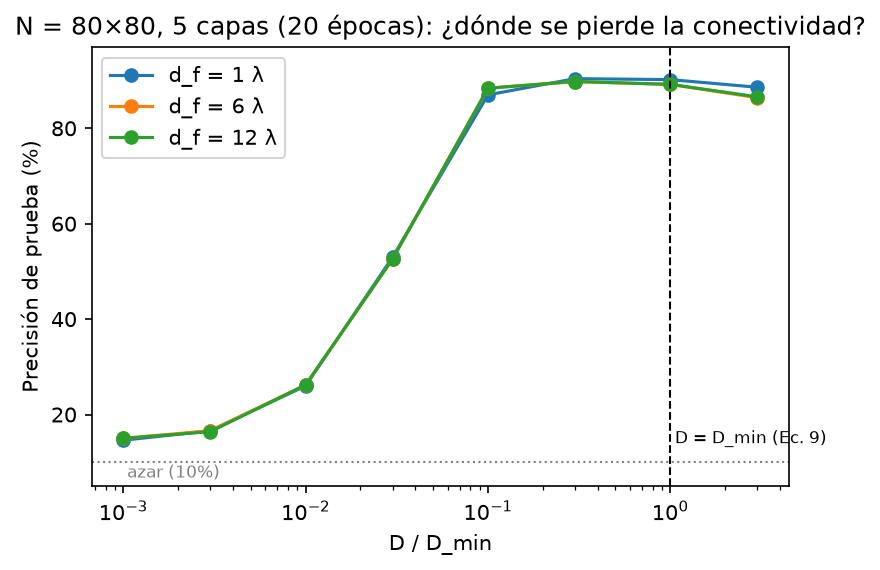
\includegraphics[width=0.72\textwidth]{sweep.png}
\caption[Barrido de conectividad]{Precisión de prueba en función de $D/\Dmin$ para
$d_f=1\lambda$, $6\lambda$ y $12\lambda$ ($\sqrt N=80$, 5 capas, 20 épocas). Las curvas coinciden y
la transición ocurre entre $0.03$ y $0.1\,\Dmin$, no en $D=\Dmin$.}
\label{fig:barrido}
\end{figure}

\begin{table}[htbp]
\centering
\caption{Precisión de prueba (\%) del barrido de conectividad (5 capas, 20 épocas).}
\label{tab:barrido}
\begin{tabular}{@{}lcccccccc@{}}
\toprule
$D/\Dmin$ & 0.001 & 0.003 & 0.01 & 0.03 & 0.1 & 0.3 & 1 & 3\\
\midrule
$d_f=1\lambda$  & 14.6 & 16.6 & 26.0 & 53.0 & 87.0 & 90.4 & 90.2 & 88.6\\
$d_f=6\lambda$  & 15.0 & 16.6 & 26.2 & 52.6 & 88.4 & 89.8 & 89.2 & 86.4\\
$d_f=12\lambda$ & 15.0 & 16.4 & 26.2 & 52.6 & 88.4 & 89.8 & 89.2 & 86.6\\
\bottomrule
\end{tabular}
\end{table}

\begin{resultado}{Conclusiones del barrido}
\begin{enumerate}
  \item \textbf{$D/\Dmin$ es la variable correcta.} Las tres curvas coinciden. Para $6\lambda$ y
  $12\lambda$ los resultados son prácticamente \emph{idénticos}, como predice \cref{prop:fresnel}: ambos
  sistemas tienen el mismo número de Fresnel por neurona y son ópticamente equivalentes. Con
  $d_f=1\lambda$, fuera del régimen paraxial, la diferencia sigue siendo menor a un punto
  en la zona de transición y alcanza hasta \num{2.2}~puntos en $D=3\,\Dmin$.
  \item \textbf{El criterio es suficiente pero unas diez veces más estricto de lo necesario.}
  Con $D=0.1\,\Dmin$ ya se alcanza el \SI{88.4}{\percent} (para $6\lambda$ y $12\lambda$), a sólo
  \num{1.4}~puntos del máximo en $0.3\,\Dmin$ (\SI{89.8}{\percent}).
  \item \textbf{Pasarse del criterio empeora.} En $D=3\,\Dmin$ la precisión baja a
  \SIrange{86.4}{88.6}{\percent} por la luz que escapa fuera de los bordes de las capas.
\end{enumerate}
\end{resultado}

Una explicación física del punto~2 es que la conectividad se \emph{acumula}: la red tiene
$L+1=6$ propagaciones y, aunque una sola no conecte bordes opuestos, la luz puede atravesar la
abertura transversal en varios saltos sucesivos. Si los radios de difracción se sumaran de
forma lineal bastaría $D\approx\Dmin/(L+1)=\Dmin/6\approx0.17\,\Dmin$; la transición observada
ocurre ligeramente antes (entre $0.03$ y $0.1\,\Dmin$).

Para comprobar esta hipótesis de \emph{conectividad acumulada}, se repitió el barrido fijando
$d_f=6\lambda$ y variando el número de capas difractivas $L\in\{1,3,5,8\}$ con 20 épocas por
punto (\cref{fig:barrido-capas,tab:barrido-capas}).

\begin{figure}[htbp]
\centering
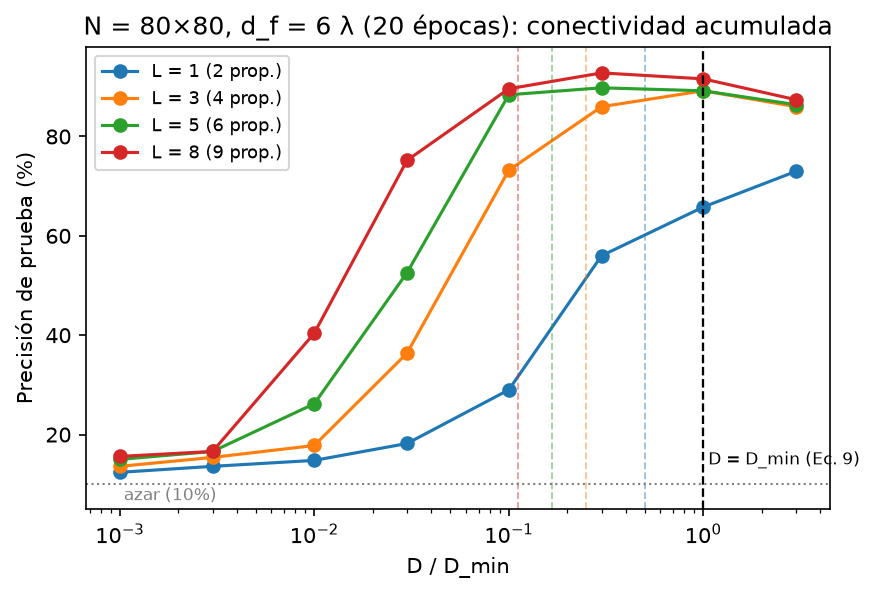
\includegraphics[width=0.72\textwidth]{sweep_layers.png}
\caption[Barrido de conectividad por número de capas]{Precisión de prueba en función de
$D/\Dmin$ para $L\in\{1,3,5,8\}$ capas ($d_f=6\lambda$, $\sqrt N=80$, 20 épocas). Las líneas
verticales punteadas de cada color indican el umbral estimado $D/\Dmin=1/(L+1)$. Al aumentar el
número de capas, la curva de transición se desplaza sistemáticamente hacia distancias menores.}
\label{fig:barrido-capas}
\end{figure}

\begin{table}[htbp]
\centering
\caption{Precisión de prueba (\%) variando el número de capas $L$ ($d_f=6\lambda$, 20 épocas).}
\label{tab:barrido-capas}
\begin{tabular}{@{}lccccccccc@{}}
\toprule
Capas $L$ ($L+1$ prop.) & $\frac{1}{L+1}$ & 0.001 & 0.003 & 0.01 & 0.03 & 0.1 & 0.3 & 1 & 3\\
\midrule
$L=1$ (2 prop.) & 0.500 & 12.4 & 13.6 & 14.8 & 18.2 & 29.0 & 56.0 & 65.8 & 73.0\\
$L=3$ (4 prop.) & 0.250 & 13.6 & 15.4 & 17.8 & 36.4 & 73.2 & 86.0 & 89.2 & 86.0\\
$L=5$ (6 prop.) & 0.167 & 15.0 & 16.6 & 26.2 & 52.6 & 88.4 & 89.8 & 89.2 & 86.4\\
$L=8$ (9 prop.) & 0.111 & 15.6 & 16.6 & 40.4 & 75.2 & 89.6 & 92.8 & 91.6 & 87.4\\
\bottomrule
\end{tabular}
\end{table}

Los resultados confirman directamente la hipótesis y revelan dos efectos acoplados:
\begin{enumerate}
  \item \textbf{Desplazamiento sistemático del umbral con $L+1$.} Al incrementar el número de
  etapas de propagación, el codo de transición se recorre hacia la izquierda en la escala
  logarítmica de $D/\Dmin$: en $D=0.03\,\Dmin$, la precisión crece monótonamente de
  \SI{18.2}{\percent} ($L=1$) a \SI{36.4}{\percent} ($L=3$), \SI{52.6}{\percent} ($L=5$) y
  \SI{75.2}{\percent} ($L=8$). De igual modo, en $D=0.1\,\Dmin$, $L=1$ apenas logra
  \SI{29.0}{\percent} y $L=3$ llega a \SI{73.2}{\percent}, mientras que $L=5$ y $L=8$ ya entran
  en la meseta de alta precisión (\SI{88.4}{\percent} y \SI{89.6}{\percent}). Esto concuerda con
  la escala $D/\Dmin\sim 1/(L+1)$, pues las máscaras sucesivas pueden dirigir haces difractados en
  ángulo acumulado a través de las $L+1$ propagaciones.
  \item \textbf{Capacidad expresiva frente a conectividad.} Con una sola capa ($L=1$), aun en
  $D=\Dmin$ y $D=3\,\Dmin$ (donde un único salto ya conecta toda la abertura), la precisión se
  estanca en \SI{65.8}{\percent} y \SI{73.0}{\percent}. Ello demuestra que, además de permitir la
  mezcla espacial por difracción, apilar varias máscaras de fase ($L\ge 3$) es indispensable para
  aumentar los grados de libertad de la transformación óptica, alcanzando \SI{92.8}{\percent} con
  $L=8$ en $D=0.3\,\Dmin$.
\end{enumerate}

\FloatBarrier
\section{Funcionamiento de la red entrenada}\label{sec:funcionamiento}

\Cref{fig:fases,fig:ejemplos,fig:corte} muestran la red del caso~2 una vez entrenada.

\begin{figure}[htbp]
\centering
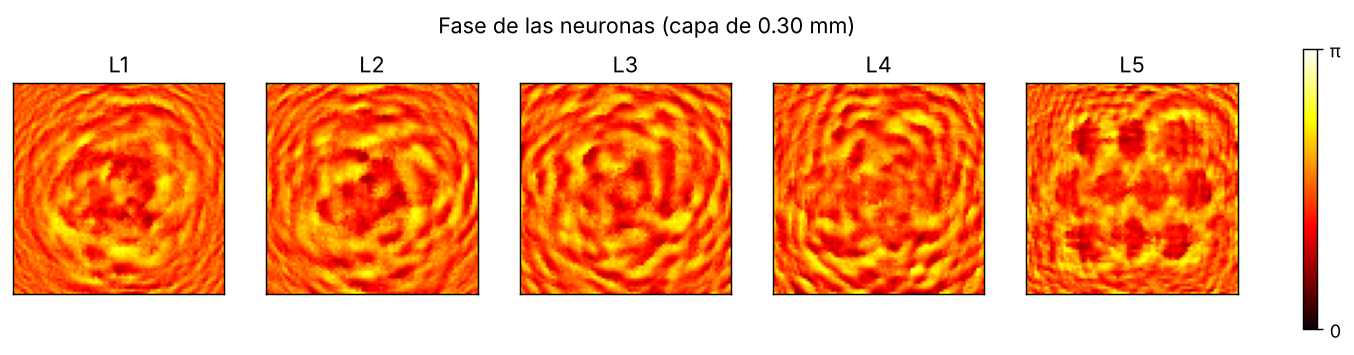
\includegraphics[width=\textwidth]{fases.png}
\caption[Fases entrenadas]{Fases de las cinco capas entrenadas (caso~2), equivalentes a la
Fig.~1(b) del artículo.}
\label{fig:fases}
\end{figure}

\begin{figure}[htbp]
\centering
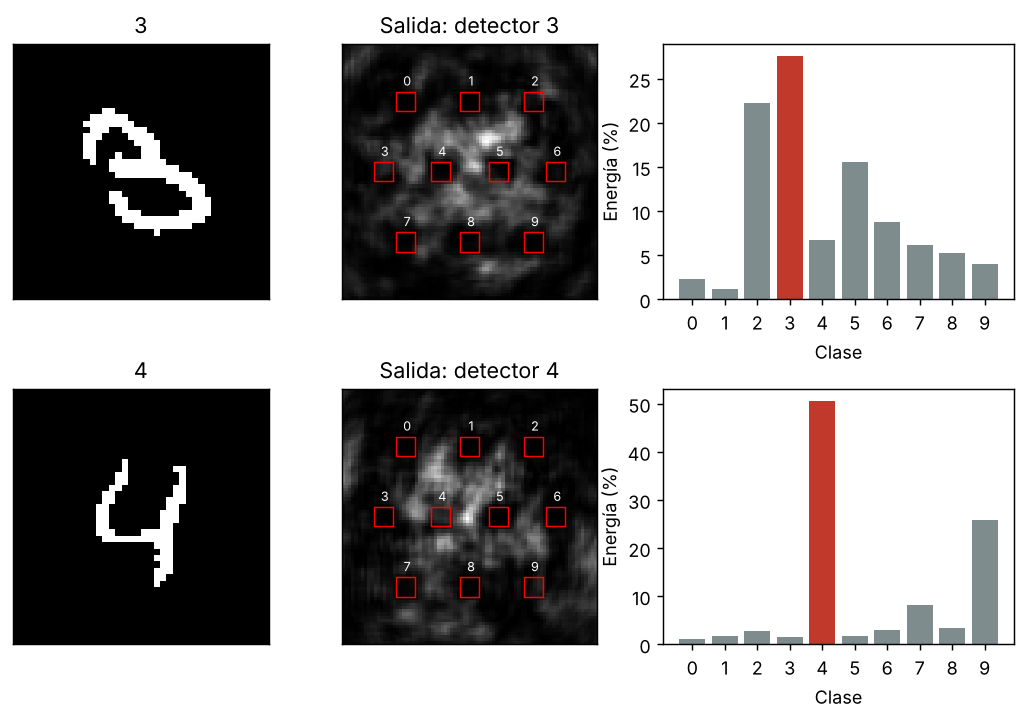
\includegraphics[width=0.9\textwidth]{fig3_ejemplos.png}
\caption[Ejemplos de clasificación]{Objeto de entrada, intensidad en el plano de salida con
los detectores y distribución de energía entre detectores, como en la Fig.~3 del artículo.}
\label{fig:ejemplos}
\end{figure}

\begin{figure}[htbp]
\centering
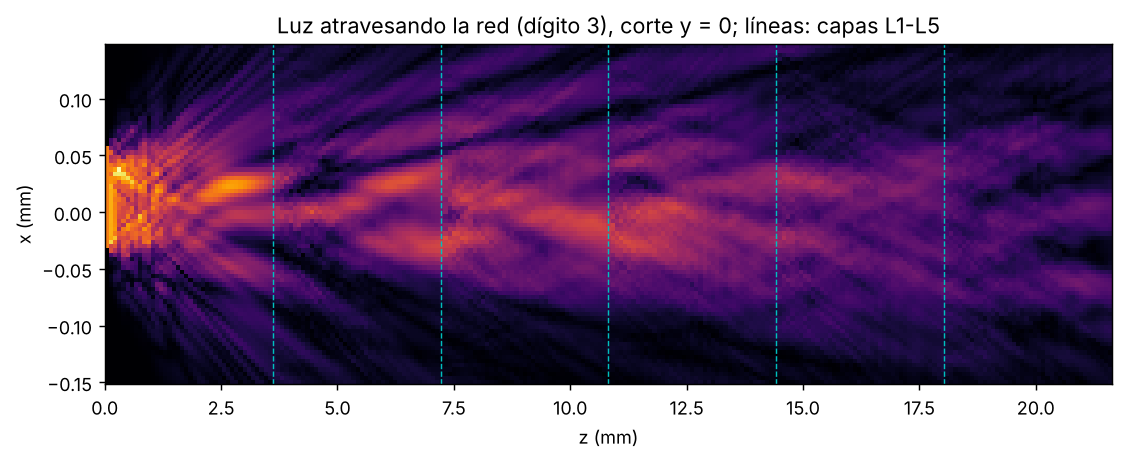
\includegraphics[width=\textwidth]{corte_xz.png}
\caption[Corte longitudinal de la intensidad]{Intensidad en el plano $y=0$ a lo largo de
todo el sistema para un dígito 3. Las líneas punteadas son las capas. La luz se redistribuye
capa a capa hasta concentrarse en el detector correcto.}
\label{fig:corte}
\end{figure}

En las máscaras de fase entrenadas (\cref{fig:fases}) se distingue una clara división funcional
entre capas. Las primeras cuatro capas (\texttt{L1}--\texttt{L4}) presentan patrones
cuasi-concéntricos de anillos y rejillas curvas de frecuencia espacial creciente: recuerdan a
placas zonales de Fresnel deformadas que reciben el haz modulado en amplitud por el dígito de
entrada y desvían sus componentes de Fourier hacia distintas regiones transversales de la
abertura de \SI{0.30}{mm}. En contraste, la última máscara (\texttt{L5}) organiza sus fases en
un arreglo explícito de diez sub-aberturas focalizadoras dispuestas exactamente en la
geometría 3--4--3 de los detectores (\cref{fig:fases}, derecha): actúa como una matriz de
microlentes difractivas que concentra la energía ya clasificada en cada caja receptora
(\cref{fig:ejemplos}).

El corte longitudinal $x\text{--}z$ en el plano $y=0$ (\cref{fig:corte}) ilustra esta evolución
espacial para un dígito~3. En $z=0$, la luz atraviesa únicamente los trazos binarios del
dígito en la región central ($|x|\lesssim\SI{0.06}{mm}$) y se expande por difracción en forma
de abanico hasta alcanzar la primera máscara (\texttt{L1}, $z\approx\SI{3.6}{mm}$). A lo largo
de \texttt{L1}--\texttt{L4} ($z\in[3.6,\,14.4]\,\si{mm}$), la modulación de fase redirige el
frente de onda para contener la energía dentro de la abertura finita y canalizarla mediante
interferencia constructiva en trayectorias oblicuas bien definidas; finalmente, después de
\texttt{L5} ($z\approx\SI{18.0}{mm}$), la intensidad converge selectivamente sobre el plano de
salida ($z\approx\SI{21.6}{mm}$) en la coordenada transversal del detector correspondiente.

\FloatBarrier
\section{Tolerancias de fabricación}\label{sec:fabricacion}

El artículo reporta \SI{91.57}{\percent} en simulación y \SI{84}{\percent} en el experimento. Para
estimar qué imperfecciones explican esa diferencia, se evaluó la red del caso~2 (neuronas de
\SI{3.8}{\micro m}) \emph{sin reentrenar} bajo cuatro tipos de error (\cref{fig:fabricacion}).

\begin{figure}[htbp]
\centering
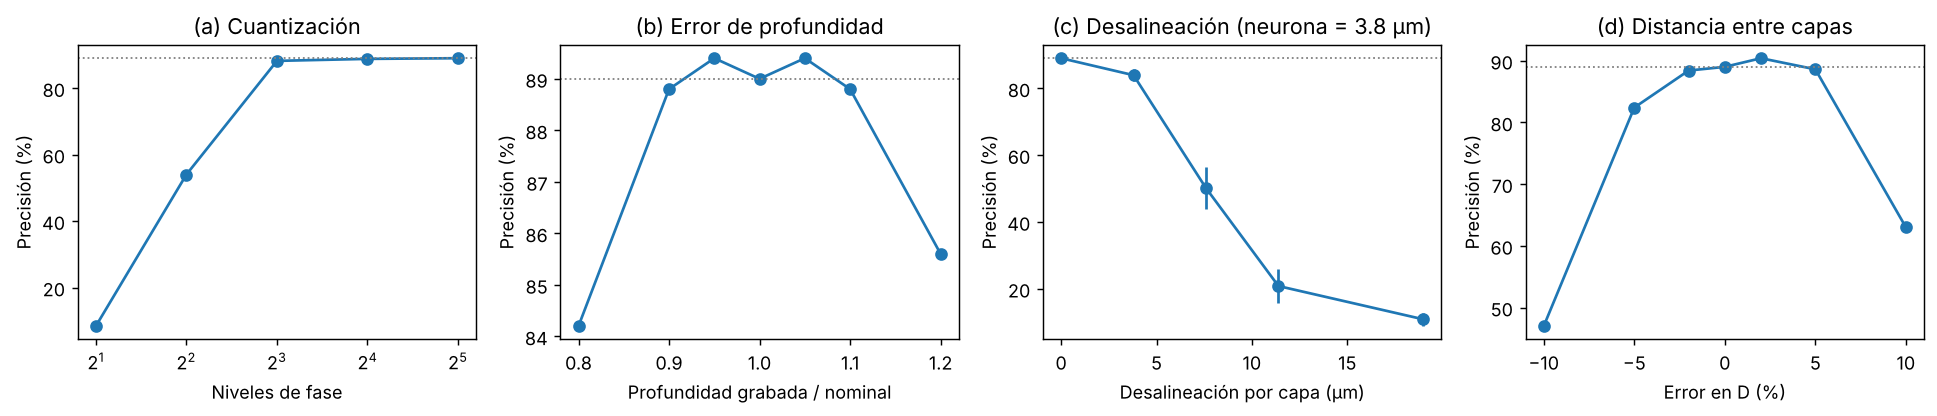
\includegraphics[width=0.90\textwidth]{fabricacion.png}
\caption[Tolerancias de fabricación]{Precisión de la red del caso~2 ante (a) cuantización
de la fase, (b) error en la profundidad grabada, (c) desalineación lateral aleatoria de cada
capa y (d) error en la distancia entre capas. La línea punteada es la red ideal
(\SI{89.0}{\percent}).}
\label{fig:fabricacion}
\end{figure}

\begin{table}[htbp]
\centering
\caption{Precisión (\%) de la red del caso~2 bajo errores de fabricación.}
\label{tab:fabricacion}
\begin{tabular}{@{}llcccccc@{}}
\toprule
\multirow{2}{*}{(a) Cuantización} & niveles & 2 & 4 & 8 & 16 & 32 & \\
 & precisión & 8.4 & 54.0 & 88.2 & 88.8 & 89.0 & \\
\midrule
\multirow{2}{*}{(b) Profundidad} & real/nominal & 0.8 & 0.9 & 0.95 & 1.05 & 1.1 & 1.2\\
 & precisión & 84.2 & 88.8 & 89.4 & 89.4 & 88.8 & 85.6\\
\midrule
\multirow{2}{*}{(c) Desalineación} & neuronas (\si{\micro m}) & 1 (3.8) & 2 (7.6) & 3 (11.4) & 5 (19.0) & & \\
 & precisión & 83.9 & 50.1 & 20.8 & 10.8 & & \\
\midrule
\multirow{2}{*}{(d) Distancia} & error en $D$ & $-10\%$ & $-5\%$ & $-2\%$ & $+2\%$ & $+5\%$ & $+10\%$\\
 & precisión & 47.0 & 82.4 & 88.4 & 90.4 & 88.6 & 63.0\\
\bottomrule
\end{tabular}
\end{table}

La malla numérica tiene una muestra por neurona, por lo que sólo pueden simularse
desplazamientos laterales de un número entero de neuronas; en cada evaluación, cada capa se
desplaza exactamente $k$ neuronas en una dirección aleatoria independiente (5 repeticiones).

\begin{resultado}{Conclusiones de fabricación}
\begin{itemize}
  \item Hacen falta al menos \textbf{8 niveles de fase} (3 pasos de litografía): con 4 niveles la
  precisión cae al \SI{54}{\percent}.
  \item La tolerancia más crítica es la \textbf{alineación lateral}: desplazar cada capa una
  sola neurona (\SI{3.8}{\micro m}) baja la precisión al \SI{83.9}{\percent}, prácticamente la
  cifra experimental del artículo, y dos neuronas la reducen al \SI{50}{\percent}.
  \item Un error de $\pm\SI{10}{\percent}$ en la profundidad apenas afecta, y la distancia entre
  capas tolera $\pm\SI{5}{\percent}$.
\end{itemize}
\end{resultado}

\FloatBarrier
\section{Sistema completo de \texorpdfstring{$1000\times1000$}{1000x1000} neuronas}\label{sec:sistema-completo}

El sistema completo del artículo consiste en 5 capas difractivas de $1000\times1000$ neuronas
($d_f=\SI{4}{\micro m}$, abertura $w=\SI{4}{mm}$, separación $D=\SI{50}{mm}\approx\Dmin$),
11 clases (dígitos 0--9 y la clase adicional~X para dígitos tapados o alterados),
\num{80000} imágenes de entrenamiento (\num{55000} de MNIST y \num{25000} modificadas) y
\num{11000} imágenes de prueba (\num{10000} y \num{1000}, respectivamente). Dado el costo de
propagar arreglos complejos rellenados de $2000\times2000$ puntos (\cref{sec:costo}), la red se
entrenó en la RTX~5060~Ti (\cref{sec:hardware}) con tamaño de lote óptimo \texttt{--bs 24}
(\num{3334} iteraciones de Adam por época) durante 6 épocas completas (\num{20004} pasos de
gradiente).

La evolución por época (\cref{tab:full-hist}) muestra una rápida convergencia inicial
(\SI{79.11}{\percent} tras la época~1 y \SI{88.32}{\percent} en la época~3) seguida de una
aproximación asintótica a la meseta en la época~6, donde la precisión de prueba alcanza
\textbf{\SI{90.63}{\percent}} en un tiempo total de \SI{10537}{s} (\SI{2}{h} \SI{56}{min}).
\Cref{tab:full} resume el desempeño frente a \textcite{chen2021}: la diferencia respecto al
\SI{91.57}{\percent} del artículo es menor a un punto porcentual (\num{0.94}~puntos porcentuales), pese a
entrenar 6 épocas en lugar de 20 y emplear nuestra propia generación sintética de la clase~X.

\begin{table}[!htbp]
\centering
\caption{Convergencia por época del sistema completo de $1000\times1000$ neuronas (\texttt{--bs 24}, RTX~5060~Ti).}
\label{tab:full-hist}
\begin{tabular}{@{}ccccc@{}}
\toprule
Época & Pérdida (train) & Precisión train (\%) & Precisión test (\%) & Tiempo acumulado\\
\midrule
1 & 1.2509 & 64.12 & 79.11 & \SI{30.0}{min}\\
2 & 0.6865 & 83.61 & 85.96 & \SI{60.3}{min}\\
3 & 0.5451 & 87.45 & 88.32 & \SI{89.5}{min}\\
4 & 0.4808 & 89.08 & 89.49 & \SI{118.2}{min}\\
5 & 0.4421 & 90.11 & 89.95 & \SI{146.9}{min}\\
\textbf{6} & \textbf{0.4156} & \textbf{90.79} & \textbf{90.63} & \textbf{\SI{175.6}{min} (\SI{2.93}{h})}\\
\bottomrule
\end{tabular}
\end{table}

\begin{table}[!htbp]
\centering
\small
\caption[Resultados del sistema completo de $1000\times1000$ neuronas]{Comparación del sistema completo ($1000\times1000$ neuronas, 11 clases) frente a \textcite{chen2021}.}
\label{tab:full}
\begin{tabularx}{\textwidth}{@{}>{\raggedright\arraybackslash}X>{\centering\arraybackslash}p{4.3cm}>{\centering\arraybackslash}p{4.3cm}@{}}
\toprule
Métrica & Artículo (20 épocas) & Este trabajo (6 épocas)\\
\midrule
Precisión total (11 clases, \num{11000} imgs.) & \SI{91.57}{\percent} & \textbf{\SI{90.63}{\percent}}\\
Dígitos sin cambio (0--9, \num{10000} imgs.) & --- & \textbf{\SI{90.24}{\percent}}\\
Clase X (tapados o alterados, \num{1000} imgs.) & --- & \textbf{\SI{94.50}{\percent}}\\
Tiempo de entrenamiento & $\approx\SI{20}{h}$ ($\approx\SI{1}{h}$/época, GTX~1080) & \SI{2.93}{h} (\SI{29.3}{min}/época, RTX~5060~Ti)\\
\bottomrule
\end{tabularx}
\end{table}

\Cref{fig:full-confusion,fig:full-fases,fig:full-ejemplos,fig:full-seises,fig:full-onda,fig:full-corte}
muestran el comportamiento óptico del modelo de $1000\times1000$ evaluado con
\texttt{05\_evaluate.py}. En la matriz de confusión (\cref{fig:full-confusion}), todas las
clases concentran su diagonal con alta pureza —destacando el dígito~1 (\num{1100} aciertos) y
la clase~X (\SI{94.50}{\percent})—, y la mayor fuente de error residual corresponde a dígitos
difíciles (como el~2 o el~5) rechazados hacia la clase~X. Las máscaras de fase
(\cref{fig:full-fases}) exhiben rejillas difractivas finas en \texttt{L1}--\texttt{L3} y
concentran progresivamente once microlentes difractivas en \texttt{L4}--\texttt{L5} siguiendo
exactamente la disposición 3--2--2--2--2 de los 11 detectores del plano de salida.

Los ejemplos individuales confirman la selectividad espacial del clasificador: un 3 o un 4
íntegros enfocan la mayor parte de la energía en su detector nominal, mientras que sus
versiones alterada o tapada redirigen el \SIrange{50}{73}{\percent} de la energía detectada
hacia la caja~X (\cref{fig:full-ejemplos}); cuatro realizaciones distintas del dígito~6
concentran de manera consistente su máximo en el detector~6 (\cref{fig:full-seises}); y una
onda plana uniforme sin dígito (\cref{fig:full-onda}) es enviada casi por completo al detector~X
($\approx\SI{89}{\percent}$), evidenciando que la red aprende a tratar cualquier patrón no
reconocible como objeto fuera de clase. El corte longitudinal $x\text{--}z$
(\cref{fig:full-corte}) muestra la expansión del frente de onda a lo largo de los
\SI{300}{mm} totales del tren óptico y su canalización hacia los haces desviados de salida.

\begin{figure}[htbp]
\centering
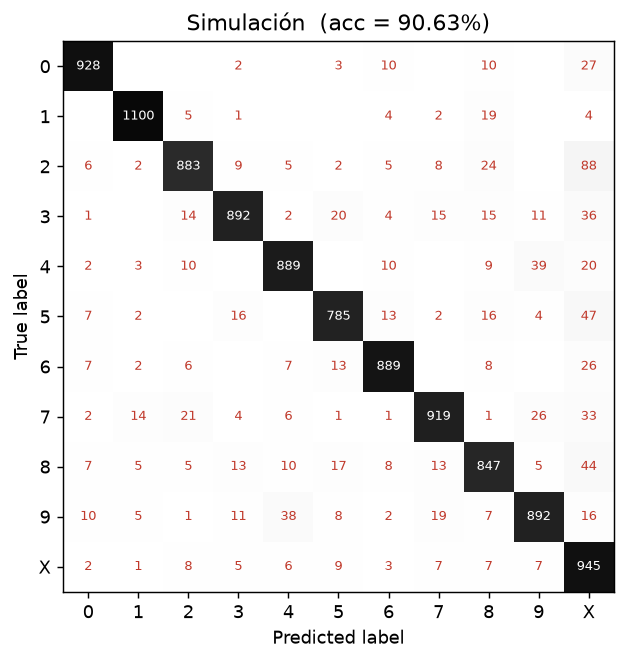
\includegraphics[width=0.62\textwidth]{full_confusion.png}
\caption[Matriz de confusión del sistema completo]{Matriz de confusión del sistema completo de
$1000\times1000$ neuronas sobre \num{11000} imágenes de prueba (precisión global del
\SI{90.63}{\percent}).}
\label{fig:full-confusion}
\end{figure}

\begin{figure}[htbp]
\centering
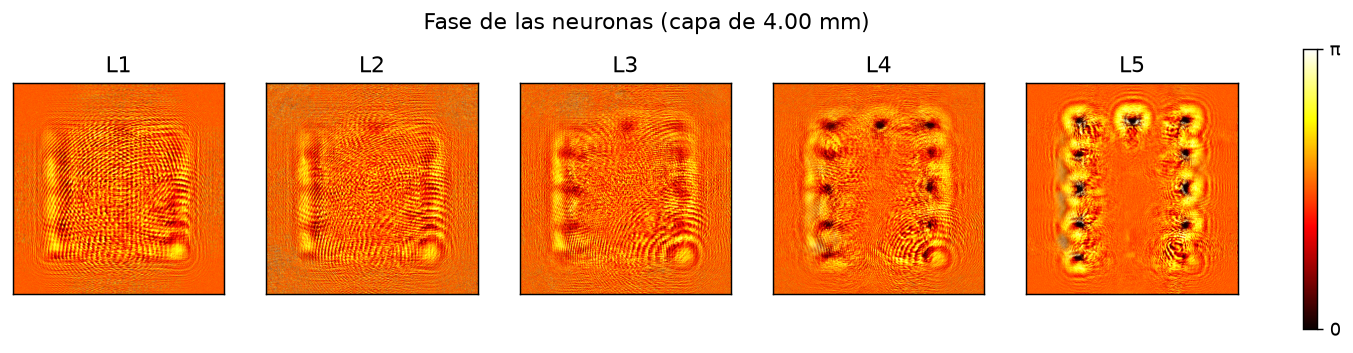
\includegraphics[width=\textwidth]{full_fases.png}
\caption[Fases entrenadas del sistema completo]{Máscaras de fase \texttt{L1}--\texttt{L5}
($4.00\times 4.00\,\si{mm}$, $1000\times1000$ neuronas) del sistema completo. En \texttt{L5}
se distinguen las 11 microlentes correspondientes al arreglo de detectores de la Fig.~3(b) del
artículo.}
\label{fig:full-fases}
\end{figure}

\begin{figure}[htbp]
\centering
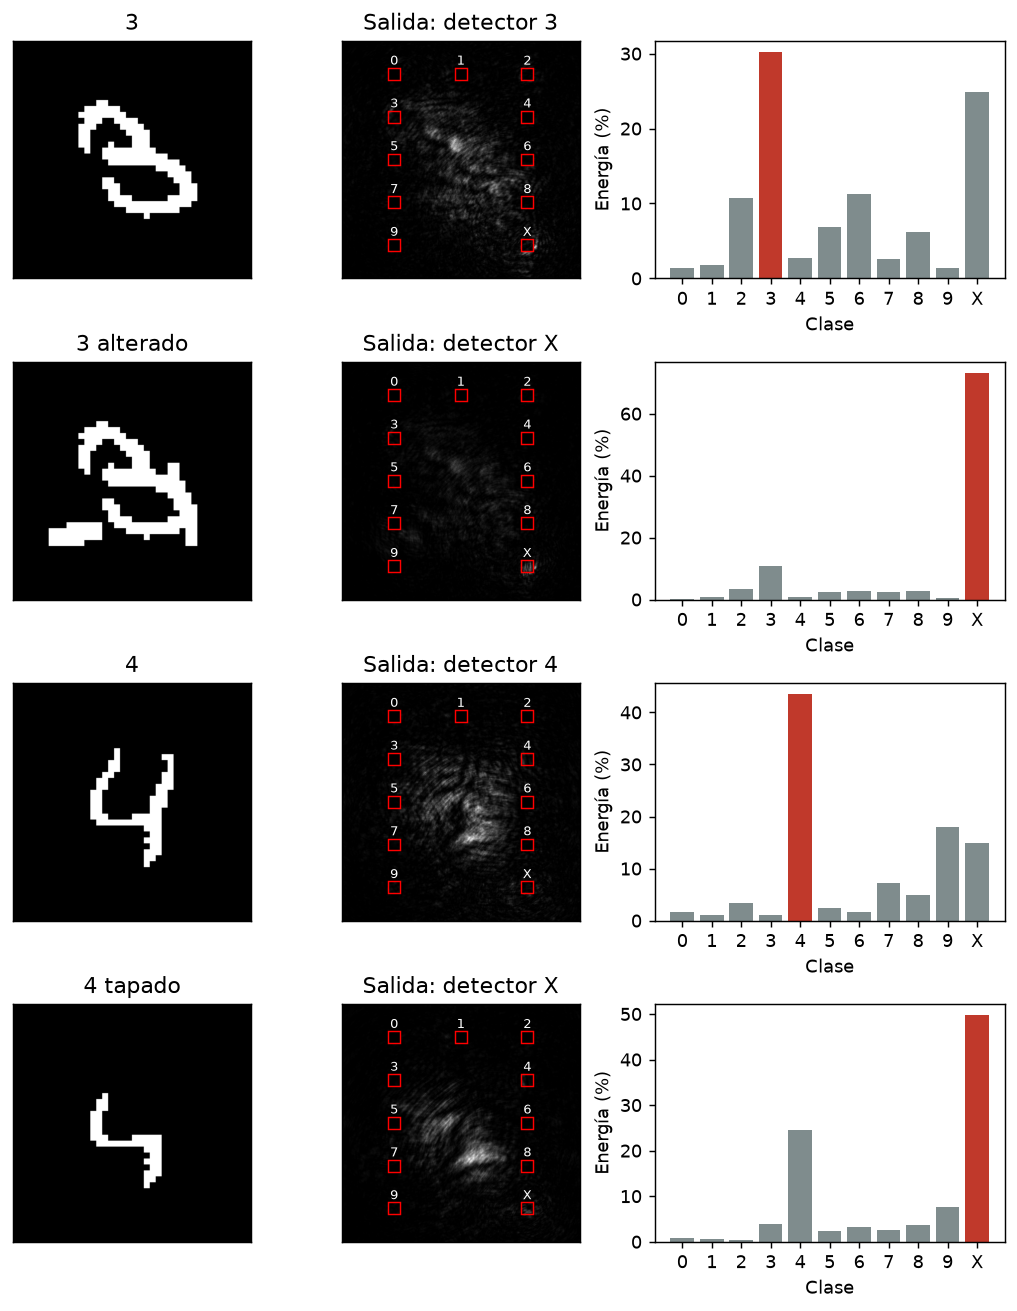
\includegraphics[width=0.88\textwidth]{full_fig3_ejemplos.png}
\caption[Ejemplos de clasificación con clase X]{Respuesta del sistema completo para un 3
intacto, un 3 alterado, un 4 intacto y un 4 tapado (equivalente a la Fig.~3 del artículo).}
\label{fig:full-ejemplos}
\end{figure}

\begin{figure}[htbp]
\centering
\begin{subfigure}{0.49\textwidth}\centering
  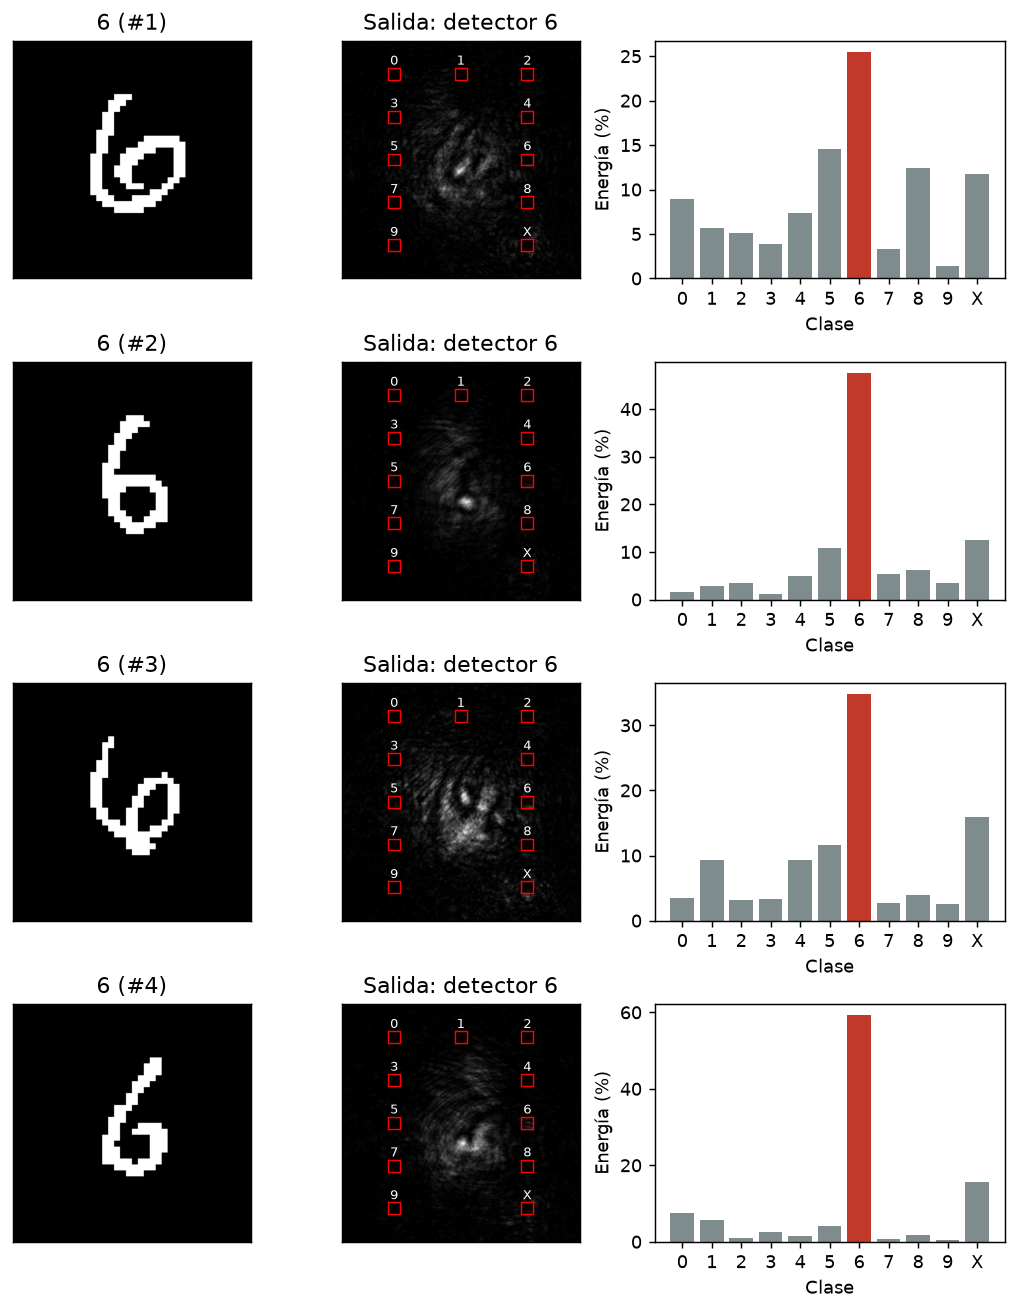
\includegraphics[width=\textwidth]{full_fig4_seises.png}
  \caption{Cuatro dígitos 6 distintos (cf.\ Fig.~4 del artículo)}
  \label{fig:full-seises}
\end{subfigure}\hfill
\begin{subfigure}{0.49\textwidth}\centering
  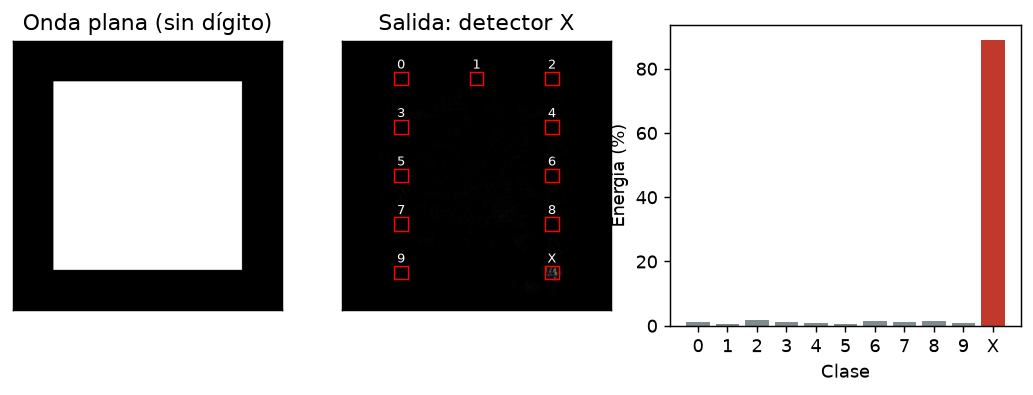
\includegraphics[width=\textwidth]{full_fig5_onda_plana.png}
  \caption{Onda plana sin dígito (cf.\ Fig.~5 del artículo)}
  \label{fig:full-onda}
\end{subfigure}
\caption[Generalización intra-clase y rechazo de onda plana]{(a) Cuatro variantes manuscritas
del dígito~6 enfocan en el detector~6; (b) una onda plana sin objeto se dirige al detector~X.}
\label{fig:full-seises-onda}
\end{figure}

\begin{figure}[htbp]
\centering
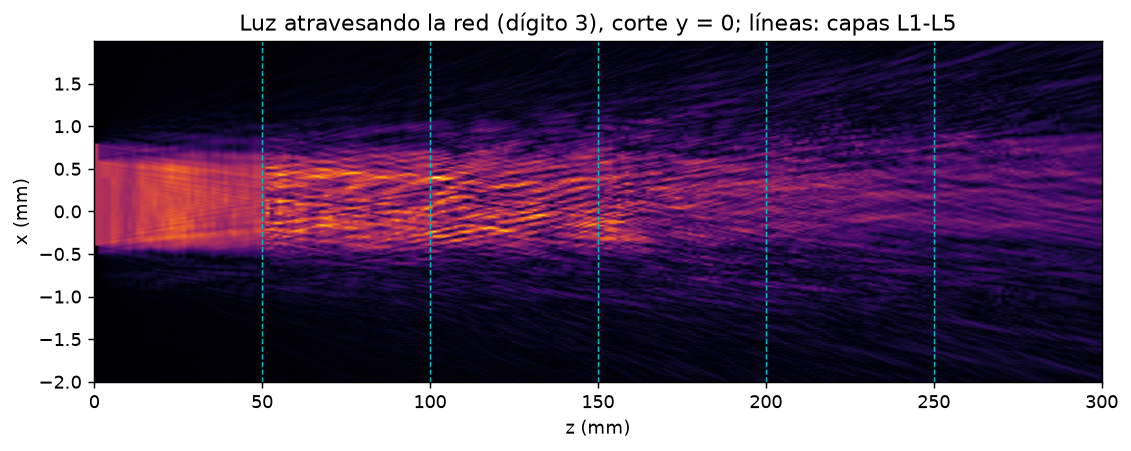
\includegraphics[width=\textwidth]{full_corte_xz.png}
\caption[Corte longitudinal del sistema completo]{Corte longitudinal $x\text{--}z$ en $y=0$
a lo largo de los \SI{300}{mm} del sistema completo para un dígito~3 (líneas punteadas en
$z=50, 100, 150, 200, 250\,\si{mm}$).}
\label{fig:full-corte}
\end{figure}

Finalmente, se repitió el análisis de tolerancias de fabricación sobre el modelo de
$1000\times1000$ en \num{2000} imágenes de prueba (\cref{fig:full-fabricacion}, línea base
ideal \SI{91.35}{\percent}). Mientras que la cuantización a 8 niveles sigue bastando con
holgura (\SI{91.05}{\percent}, e incluso 4 niveles conservan \SI{87.50}{\percent}) y los
errores de profundidad de $\pm\SI{10}{\percent}$ mantienen \SIrange{89.65}{91.70}{\percent}, la
sensibilidad a la distancia axial $D$ se vuelve mucho más severa que en el caso~2 de
$80\times80$: una desviación de $\pm\SI{2}{\percent}$ en $D=\SI{50}{mm}$ ($\pm\SI{1}{mm}$) hace
caer la precisión a \SIrange{12.05}{15.05}{\percent}. La razón cuantitativa es la siguiente.

\paragraph{Tolerancia axial.} Un error $\Delta D$ en la distancia multiplica el espectro de
cada capa por $H(u,v;\Delta D)\approx e^{\jj k\Delta D}\,e^{-\jj\pi\lambda\Delta D(u^2+v^2)}$
(\cref{eq:fresnel-tf}). En el borde de la banda controlable, $u=1/(2d_f)$, el error de fase
es $\pi\lambda\Delta D/(4d_f^2)$. Exigir que no supere $\pi/2$ da
\begin{equation}
  \Delta D\le\frac{2d_f^2}{\lambda}
  \qquad\Longrightarrow\qquad
  \frac{\Delta D}{D}\le\frac{2d_f^2}{\lambda D}=2N_{F,n}\approx\frac{1}{\sqrt N}\,\frac{\Dmin}{D},
  \label{eq:tol-axial}
\end{equation}
donde se usó \eqref{eq:dmin-paraxial}. La tolerancia relativa decrece como $1/\sqrt N$:
\begin{center}
\begin{tabular}{@{}lccc@{}}
\toprule
Sistema & $2d_f^2/\lambda$ & $D$ & $\Delta D/D$ tolerable\\
\midrule
Caso 2 ($\sqrt N=80$) & \SI{45.6}{\micro m} & \SI{3.6}{mm} & \SI{1.3}{\percent}\\
Completo ($\sqrt N=1000$) & \SI{50.6}{\micro m} & \SI{50}{mm} & \SI{0.10}{\percent}\\
\bottomrule
\end{tabular}
\end{center}
Esto explica por qué el caso~2 tolera $\pm\SI{2}{\percent}$ mientras que en el sistema completo
el mismo error relativo, unas 20 veces la tolerancia, lleva la precisión al nivel del azar:
\textbf{redes más grandes, separadas cerca de $\Dmin$, son proporcionalmente más sensibles a la
distancia entre capas.}

En cuanto a la alineación lateral, desplazar cada capa una sola neurona (\SI{4}{\micro m})
reduce la precisión del sistema completo a \SI{81.4 \pm 3.5}{\percent}; dos neuronas, a
\SI{38.4 \pm 19.5}{\percent}; y tres o más la llevan al nivel del azar
(\SIrange{8.7}{12.8}{\percent}). Al igual que en el caso~2, una neurona de desalineación basta
para explicar la diferencia entre la precisión simulada y la experimental del artículo.

\begin{figure}[htbp]
\centering
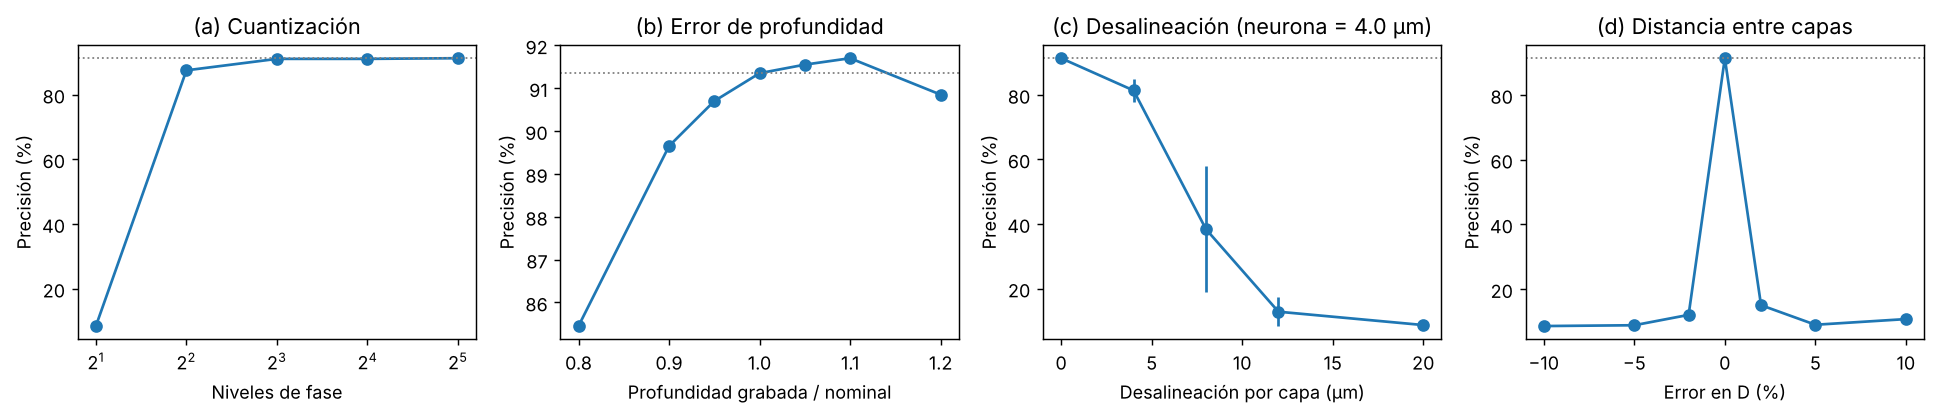
\includegraphics[width=0.88\textwidth]{full_fabricacion.png}
\caption[Tolerancias de fabricación del sistema completo]{Sensibilidad del sistema de
$1000\times1000$ neuronas (precisión ideal de \SI{91.35}{\percent} en \num{2000} imágenes) ante
(a) cuantización, (b) error de profundidad, (c) desalineación lateral y (d) variación porcentual
de $D=\SI{50}{mm}$.}
\label{fig:full-fabricacion}
\end{figure}

\FloatBarrier
\subsection{Eficiencia de detección}\label{sec:eficiencia}

La pérdida \eqref{eq:perdida} usa la energía \emph{relativa} entre detectores, así que no
premia que la luz llegue a ellos. Midiendo la eficiencia
$\eta=\sum_kE_k/\iint|Y^{\text{sal}}|^2$, sólo el \SI{1.1}{\percent} de la luz de salida del
sistema completo cae en los detectores (\SI{1.6}{\percent} en el caso~2), menos que la
fracción del plano que ocupan (\SI{2.75}{\percent} y \SI{5.6}{\percent}). La red clasifica bien,
pero en un experimento con ruido de fondo esa eficiencia sería un problema.

Añadiendo a la pérdida un término $w\,(1-\eta)$ se obtiene un compromiso entre precisión y
eficiencia (caso~2, 20 épocas):
\begin{center}
\begin{tabular}{@{}lcccc@{}}
\toprule
Peso $w$ & 0 & 1 & 3 & 10\\
\midrule
Precisión (\%) & 89.0 & 88.6 & 85.8 & 64.6\\
Eficiencia $\eta$ (\%) & 1.6 & 2.2 & 18.6 & 89.4\\
\bottomrule
\end{tabular}
\end{center}
Con $w=3$ la eficiencia se multiplica por 11 a cambio de 3 puntos de precisión.
